\section{Introduction}
\label{sec:introduction}

% state the learning objective 

\indent

The objective of this laboratory assignment is to study a circuit containing two voltage and current sources connected to various resistors. The two current sources (one dependent, $I_b$,  and one independent, $I_d$), and two voltage sources (one dependent, $V_c$,  and one independent, $V_a$) connect to 7 different resistors ($R_{1-7}$). The circuit can be seen in Figure~\ref{fig:rc}.



In Section~\ref{sec:analysis}, a theoretical analysis of the circuit is
presented. In Section~\ref{sec:simulation}, the circuit is analysed by
simulation, and the results are compared to the theoretical results obtained in
Section~\ref{sec:analysis}. The conclusions of this study are outlined in
Section~\ref{sec:conclusion}.

\begin{figure}[h] \centering
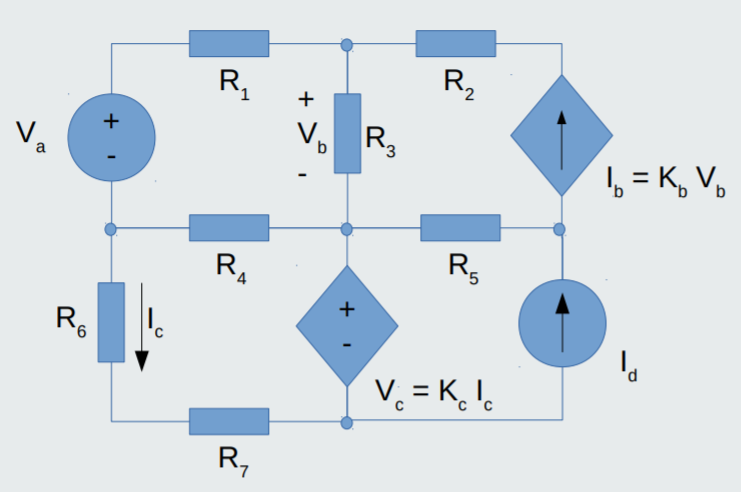
\includegraphics[width=0.8\linewidth]{Images/Circuit.png}
\caption{Voltage and Current driven circuit with 7 resistors.}
\label{fig:rc}
\end{figure}

